%% !TeX root = main.tex
\chapter{Binary Neural Networks (BNNs)}
\label{chapter:BNN}

\section{Overview}
Binary (or Binarized) Neural Networks have emerged as compact, yet powerful, neural network architectures for embedded deep learning. At their core, BNNs operate with binary weights and activations rather than full precision values as in typical deep neural networks. This fundamental shift not only simplifies computations but also introduces a range of advantages that address challenges in modern AI systems. 

The goal of this chapter is to introduce Binary Neural Networks and provide an understanding as to how these types of networks function. It will begin by motivating the development of BNNs with a discussion of the benefits these networks provide in regards to efficiency and memory consumption. Next, the basic operations and concepts behind BNNs success will be explained to give readers an idea of how binary values are created and used within the network. Following this, the chapter will move onto the two main stages involved in model inference and training, forward and backward propagation, and discuss how BNNs address the  challenges that arise as a result of using only binary values. 

\begin{figure}[htbp]
\centerline{\includegraphics[scale = .75]{images/network.png}}
\caption{High-level depiction of BNN \cite{paperExplained}}
\label{fig:network}
\end{figure}


\section{Motivation}

The development of BNNs has largely been driven by the need for more efficient architectures, particularly in resource-constrained environments. Because traditional deep neural networks use floating-point precision, the significant computational resources (i.e. many GPUs) and memory capacities required for training and storing the model are often on a scale that is infeasible for small devices. BNNs, however, are able to drastically reduce the computational complexity and memory footprint by employing binary values and bitwise operations, making them particularly well-suited for deployment in edge devices, IoT applications, and other scenarios where resources are limited. 

The operational mechanisms of BNNs involve specialized binary operations including XNOR and population count (pop count) which facilitate efficient forward and backward propagation, the details of which will be discussed in the sections that follow. By swapping normal matrix multiplication with these bitwise operations, BNNs act as a binary circuit and consequently, are particularly hardware-friendly and ideal for deployment in FPGAs and other hardware devices. 

Compare, for instance, a 32 bit floating point value which is used in most deep neural networks to a single bit used in BNNs. The single bit representation uses 1/32 of the space required by the 32 bit representation making it 32 times more memory efficient. Further, bitwise operations can typically be executed in a single clock cycle in hardware as opposed to the tens of cycles often required for computation with floating point numbers, offering significant speedup. Such improved efficiency translates to accelerated inference times and enables BNNs to be used for applications requiring real-time decision-making.

%\newpage

% \begin{figure}[htbp]
% \centerline{\includegraphics[scale = .75]{network.png}}
% \caption{}
% \label{fig2}
% \end{figure}

\section{Binary Values}

The binary values in BNNs can be either one of the following combinations:
\begin{itemize}
    \item 0 and 1
    \item -1 and 1
\end{itemize}

However, -1 and 1 is much more common in practice.

\begin{exercise}
Can you guess why this may be the case? Think about how logical operation, specifically XNOR, could relate to multiplication. The answer will become clear in the sections that follow.
\end{exercise} 


\section{Binary Operations}
\subsection{XNOR}
The XNOR (exclusive NOR) gate is a digital logic gate that acts as an XOR (exclusive or) operation followed by an inverter. As seen in the table below its output is “true” if the inputs are the same and “false” otherwise. In the context of BNNs, the XNOR operation is applied element-wise between binary inputs and binary weights. The resulting binary output indicates whether the input and weight have the same or different sign. \\ 

\begin{figure}[htbp]
\centerline{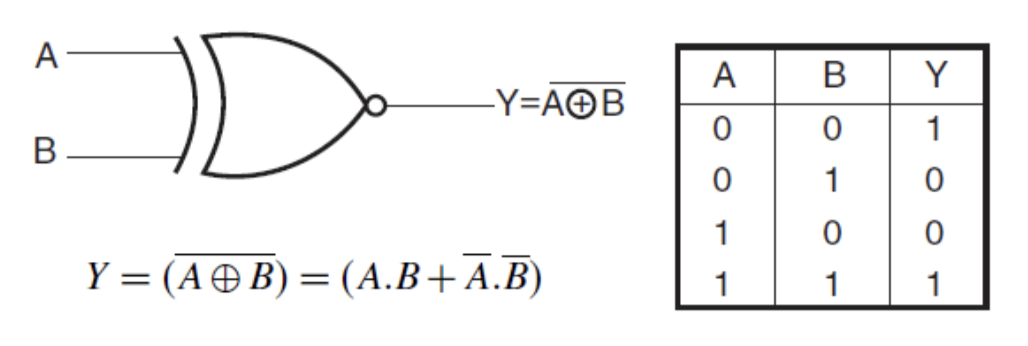
\includegraphics[scale = .65]{images/xnor.png}}
\caption{XNOR logic gate and truth table.}
\label{fig:xnor}
\end{figure}

\newpage

It was mentioned previously that using -1 and 1 as the binary values in a BNN was preferred over 0 and 1. The reason for this lies in the XNOR operation. Consider two binary inputs $A \in \{0,1\}$ and $B \in \{0,1\}$ and perform the XNOR operation on these values. Then, map 0 to -1 and 1 to +1 so that $A \in \{-1,+1\}$ and $B \in \{-1,+1\}$ and perform multiplication on these values.

%\newpage

\begin{figure}[htbp]
\centerline{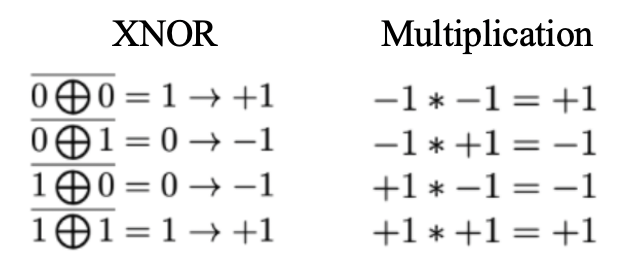
\includegraphics[scale = .65]{images/comparison.png}}
\label{fig:comparison}
\end{figure}


Notice that the output for these two operations is the same. Thus, when using binary values of -1 and +1 the XNOR operation is simply multiplication, demonstrating how we can replace costly arithmetic operations with bitwise operations in BNNs. 


\subsection{Population Count}
The population count (popcount) operation counts the number of bits set to 1 in a binary vector. In BNNs, pop count operations help determine binary activations during the forward pass by quantifying the number of positive weights in a given layer. 

\subsection{XNOR and Popcount for Matrix Multiplication}
In combination, XNOR and popcount operations can replace normal MAC (multiply-accumulate) operations in BNNs. Below is the general formula for multiplying two binary vectors $A$ and $B$ using XNOR and popcount.

\begin{equation}
    A \cdot B = sum - (N-sum) = 2*sum - N 
\end{equation}

where, 
\begin{equation}
sum = popcount(\overline{A \oplus B}) \\
\end{equation}\\


Here, $sum$ is the number of +1's in the dot product result, $N$ is the total number of bits of the XNOR result, and $N-sum$ is the number of -1's in the dot product result. \\

\subsubsection{Example}
Let's take a look at an example to convince you of the equivalence of matrix multiplication and the XNOR popcount operations. \\

Consider two input vectors $[10, -10, -5, 9, -8, 2, 3, 1, -11]$ and $[12, -18, -13, -13, -14, -15, 11, 12, 13].$ We first binarize these using the sign function (defined in the next section) to convert our values to -1 or +1 and obtain $[1, -1, -1, 1, -1, 1, 1, 1, -1]$ and $[1, -1, -1, -1, -1, -1, 1, 1, 1]$. Then we perform both matrix multiplication (dot product) and XNOR with popcount and compare the results. Note that in order to use XNOR the values were first quantized to 0s and 1's. As depicted in the graphic on the next page, it is clear that both operations result in the same final output value of $3$. \\

\begin{figure}[htbp]
\centerline{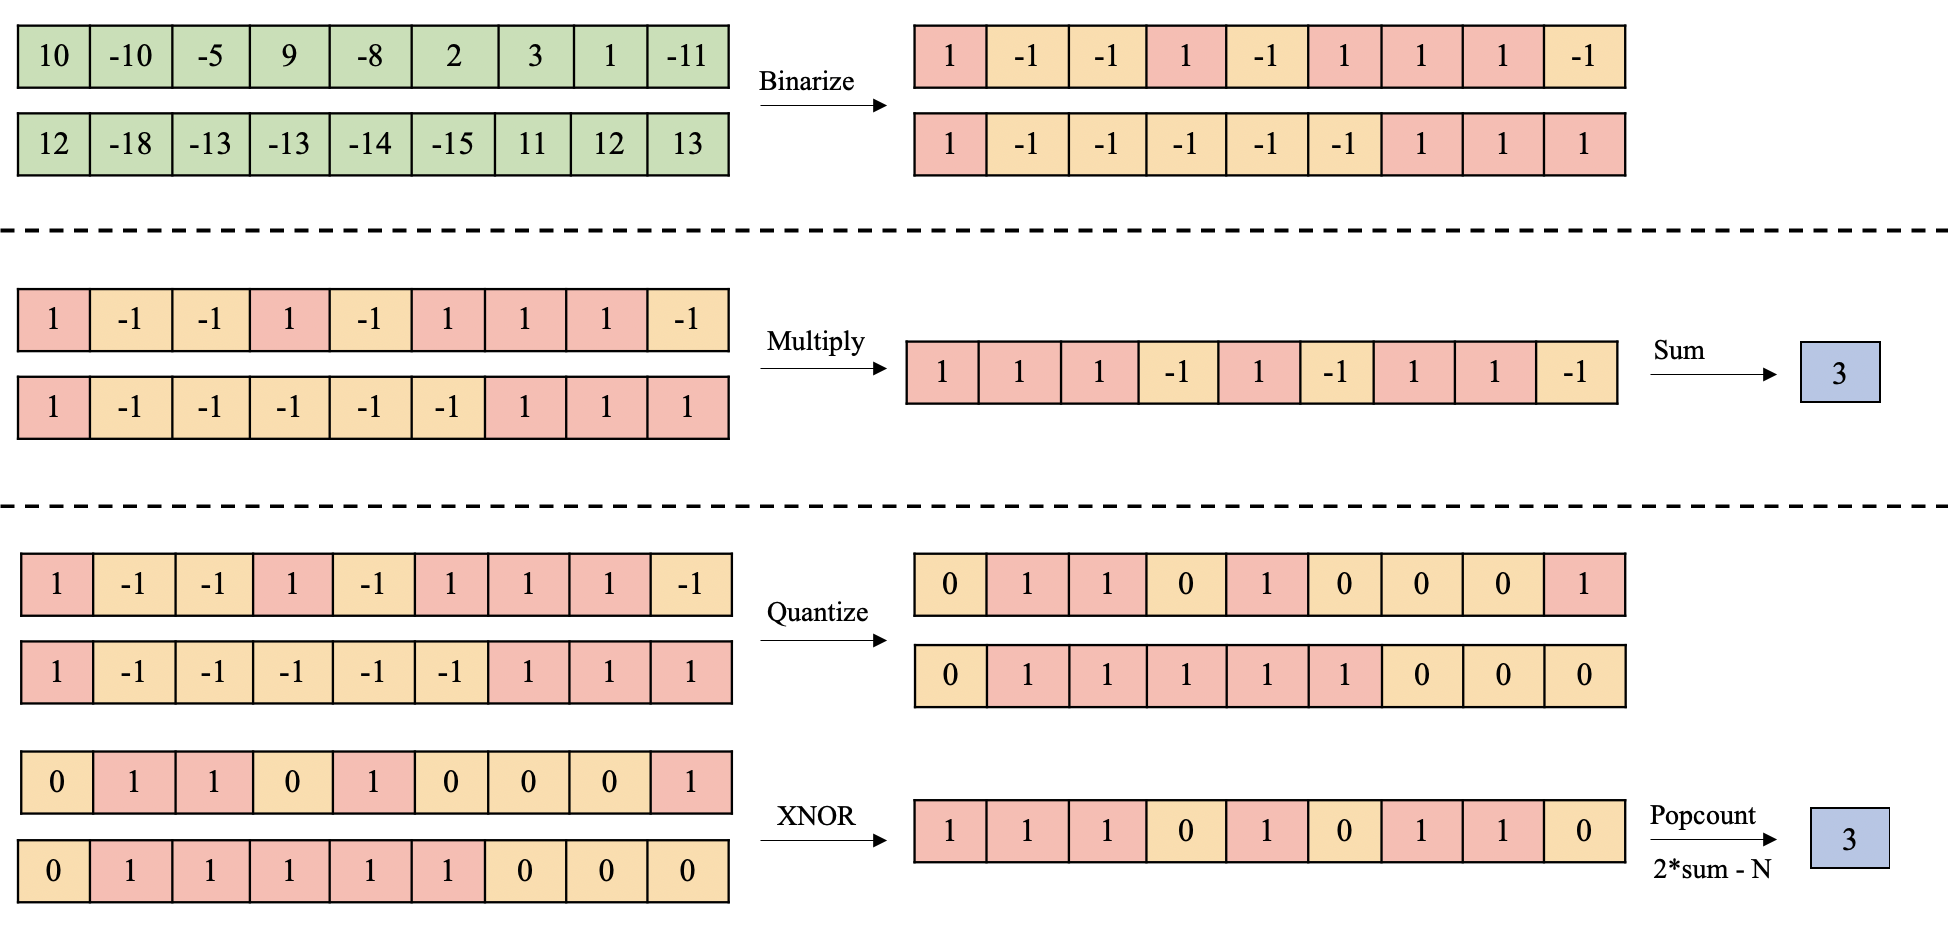
\includegraphics[scale = .50]{images/example.png}}
\label{fig:examplebnn}
\caption{Example of normal MAC vs XNOR and popcount operations.}
\end{figure}

%\newpage

\section{Binarization of the Network}
In order to achieve the benefits of using binary values in-place of floating point values discussed above, we need a way to ``binarize''
 our network. There are two binarization functions that can be used to convert the neural network's floating point values into binary values of -1 or 1. 

The first is the deterministic signum or sign function which, as the name suggests, maps real-values to -1 or 1 based on their sign. The sign function is defined as:

\begin{equation}
x^{b} = Sign(x) =
    \begin{cases}
        +1 & \text{if } x \geq{0} \\
        -1 & \text{otherwise }
    \end{cases}
\end{equation}

where $x^{b}$ is the binarized weight or activation and x is the original floating point value. 
\newpage

The second binarization function is stochastic and is defined as:

\begin{equation}
x^{b} = Sign(x) =
    \begin{cases}
        +1 & \text{with probability} p = \sigma(x) \\
        -1 & \text{with probability } 1-p
    \end{cases}
\end{equation}

where $\sigma$ is:
\begin{equation}
    \sigma (x)= max(0, min(1, \frac{x+1}{2})
\end{equation}
\\

Although the stochastic binarization can be esspecially effective in dealing with variability in data as compared to the deterministic case, it is harder to implement as it requires the hardware to generate random bits when quantizing. As a result, the deterministic sign function is more often used in practice and is what should used in your BNN project. 

\begin{exercise}
What classification tasks would perform better with stochastic binarization? Could we achieve the same performance with deterministic binarization if we add more layers?
\end{exercise}

%\newpage

\section{Forward Propagation}
Recall that in deep learning, forward propagation refers to model inference. That is, given an input, use the model's learned parameters to predict the output. For BNNs, the forward pass is similar to that of any typical deep neural networks architecture with the exception that all weights and activations are binarized to either -1 or +1. 

\subsection{General BNN Forward Propagation Psuedo Code}
The pseudo code for forward propagation of a BNN is shown below. Note that the superscript $b$ on a variable indicates that that variable is binarized. 

For layers $1$ through $L$, the weights are first binarized (and quantized) using the sign function. This step is only necessary during training, however, since once the model is fully trained only the binary weights will be stored. Then, our binary activations from the previous layer and binary weights are multiplied using the XNOR and popcount operations resulting in a non-binary sum. Following this, batch normalization is applied, if necessary, with parameters $\theta_k$. If it is not the last layer of the network, then activations are once again binarized and the process is repeated. 

\begin{figure}[htbp]
\centerline{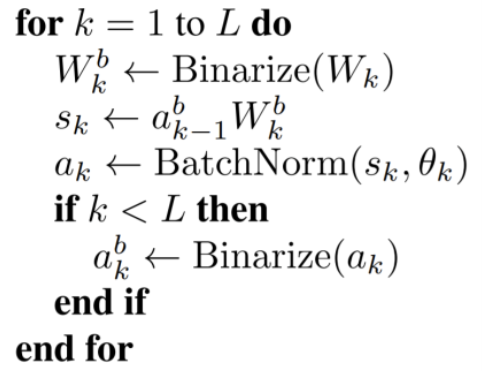
\includegraphics[scale = .65]{images/forward.png}}
\caption{Pseudo code for BNN forward propagation}
\label{fig:forward}
\end{figure}

\subsection{BNN Forward Propagation Implementation using XNOR and Popcount}
Below you will find a sample python implementation of the forward pass function provided as part of the BNN class project. This network takes a 28x28 MNIST image as input and classifies the digit depicted in the images from 0-9. Since the model was already trained, stored weights (``fc1w\_qntz'', ``fc2w\_qntz'', ``fc3w\_qntz'') are binary. There are only three layers to this BNN, with each implementing the process described in the pseudo code above: (1) Inputs to each layer (i.e. activations from the previous layer) are binarized and quantized.(2) These inputs are then multiplied with the binary weights using XNOR + popcount.(3) The output is fed to the next layer or used to make the final prediction. For the project, you will be tasked will implementing the feed\_forward\_quantized function in HLS. \\


\begin{python}
def feed_forward_quantized(self, input):
    #param input: MNIST sample input
    
    # layer 1
    X0_input = self.quantize(self.sign(self.adj(input)))
    layer1_output = self.matmul_xnor(X0_input, self.fc1w_qntz.T)
    layer1_activations = (layer1_output * 2 - 784)

    # layer 2
    layer2_input = self.sign(layer1_activations)
    layer2_quantized = self.quantize(layer2_input)
    layer2_output = self.matmul_xnor(layer2_quantized, self.fc2w_qntz.T)
    layer2_activations = (layer2_output * 2 - 128)

    # layer 3
    layer3_input = self.sign(layer2_activations)
    layer3_quantized = self.quantize(layer3_input)
    layer3_output = self.matmul_xnor(layer3_quantized, self.fc3w_qntz.T)

    final_output = (layer3_output * 2 - 64)
    A = np.array([final_output], np.int32)
        
    return A

\end{python}

\subsection{BNN Forward Propagation Implementation Using MAC}

For comparison, we have included a BNN forward propagation implementation using multiply and accumulate (MAC) rather than the XNOR and popcount introduced above. We hope it is now clear that this implementation is significantly more costly to implement in hardware. \\

\begin{python}
def feed_forward(self, input):
     """This BNN using normal MAC.
    """
    # layer 1
    X0_q = self.sign(self.adj(input))
    X1 = np.matmul(X0_q, self.fc1w_q.T)

    # layer 2
    X1_q = self.sign(X1)
    X2 = np.matmul(X1_q, self.fc2w_q.T)

    # layer 3
    X2_q = self.sign(X2)
    X3 = np.matmul(X2_q, self.fc3w_q.T)

    return X3
\end{python}


\subsection{BNN Forward Propagation Implementation in C++, Quantized}

Below we have included the feed\_forward\_quantized function in C++, for use in HLS. 
Firstly, we establish our helper functions. These include a function for executing the XNOR operation, another for the sign operation, a function for the quantize operation, and one for conducting matrix multiplication utilizing the XNOR operation. The primary feed-forward function is denoted as feed\_forward\_quantize(), designed for a two-layer Binary Neural Network (BNN). It is important to observe that flattened weight matrices are employed, and the dimensions of the original square matrices are supplied as parameters.

\begin{lstlisting}
#include <iostream>
#include <cmath>

int XNOR(int a, int b) {
    return (a == b) ? 1 : 0;
}
void matmul_xnor(int* A, int* B, int* res, int rowsA, int rowsB, int colsB) {
    for (int x = 0; x < colsB; ++x) {
        int cnt = 0;
        for (int y = 0; y < rowsA; ++y) {
            cnt += XNOR(A[y], B[y * colsB + x]);
        }
        res[x] = cnt;
    }
}
int quantize(int x) {
    return (x == 1) ? 0 : 1;
}
int sign(int x) {
    return (x > 0) ? 1 : -1;
}

void feed_forward_quantized(int* X, int* w1, int* w2, 
                            int X_size, 
                            int rowsW1, int colsW1, 
                            int rowsW2, int colsW2,
                            int* layer1_activations, int* layer2_activations) {

    // ********** Layer 1 **********
    // Quantize inputs
    int X0_input[X_size];
    for (int i = 0; i < X_size; ++i) {
        X0_input[i] = quantize(sign(X[i]));
    }
    // Perform matrix multiplication with W1 using XNOR
    matmul_xnor(X0_input, w1, layer1_activations, X_size, rowsW1, colsW1);
    for (int i = 0; i < colsW1; ++i) {
        layer1_activations[i] = (layer1_activations[i] * 2 - X_size);
    }
    // ********** Layer 2 **********
    // Quantize layer 1 activations
    int layer2_quantized[colsW1];
    for (int i = 0; i < colsW1; ++i) {
        layer2_quantized[i] = quantize(sign(layer1_activations[i]));
    }
    // Perform matrix multiplication with W2 using XNOR
    matmul_xnor(layer2_quantized, w2, layer2_activations, colsW1, rowsW2, colsW2);
    for (int i = 0; i < colsW2; ++i) {
        layer2_activations[i] = (layer2_activations[i] * 2 - colsW1);
    }
    // final output is layer2_activations
}

int main() {
    // Example usage:
    int input[] = { 1, 1 };
    int W1[] = {1, 1, 1, 1};
    int W2[] = {1, 0, 1, 1, 1, 0};
    int X_size = 2;
    int rowsW1 = 2;
    int colsW1 = 2;
    int rowsW2 = 2;
    int colsW2 = 3;
    int layer1_activations[colsW1];
    int layer2_activations[colsW2];

    feed_forward_quantized(input, W1, W2, X_size, rowsW1, colsW1, rowsW2, colsW2,
                            layer1_activations, layer2_activations);
    return 0;
}
\end{lstlisting}


\section{Back Propagation}

Backpropagation (short for ``backwards propagation of errors'') is a fundamental algorithm used to train supervised learning algorithms - BNNs being one of them. At the end of the forward pass (forward propagation), the network computes the loss (error) by comparing its outputs to the ground truth values using a loss function such as mean squared error for regression tasks or cross-entropy for classification tasks. The algorithm then calculates the gradient of the loss function with respect to each weight in the network by applying the chain rule.

\begin{exercise}
Can you think of any issue with taking the gradient here? Remember in forward propagation, we used Sign(x) to binarize weights. What does the derivative look like for this function?
\end{exercise} 

\subsection{Gradient Decent Update Rule}

Backpropagation gets its name from the fact that this chain rule process starts at the output layer and works backward through the network. The weights are then updated to minimize the loss (error) function, shown below with W the weight to update, J the loss function, and $\alpha$ the learning rate. This update process is called gradient decent.

\begin{figure}[htbp]
\centerline{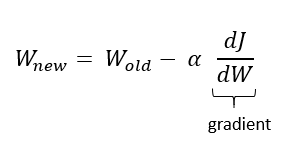
\includegraphics[scale = .65]{images/grad_decent.png}}
\caption{Gradient decent update rule.}
\label{fig:grad_descent}
\end{figure}

This process of forward and backward propagation is repeated for many iterations, updating the weights of the network each time to minimize the loss function. Below is a graphical depiction of BNN training.

\begin{figure}[htbp]
\centerline{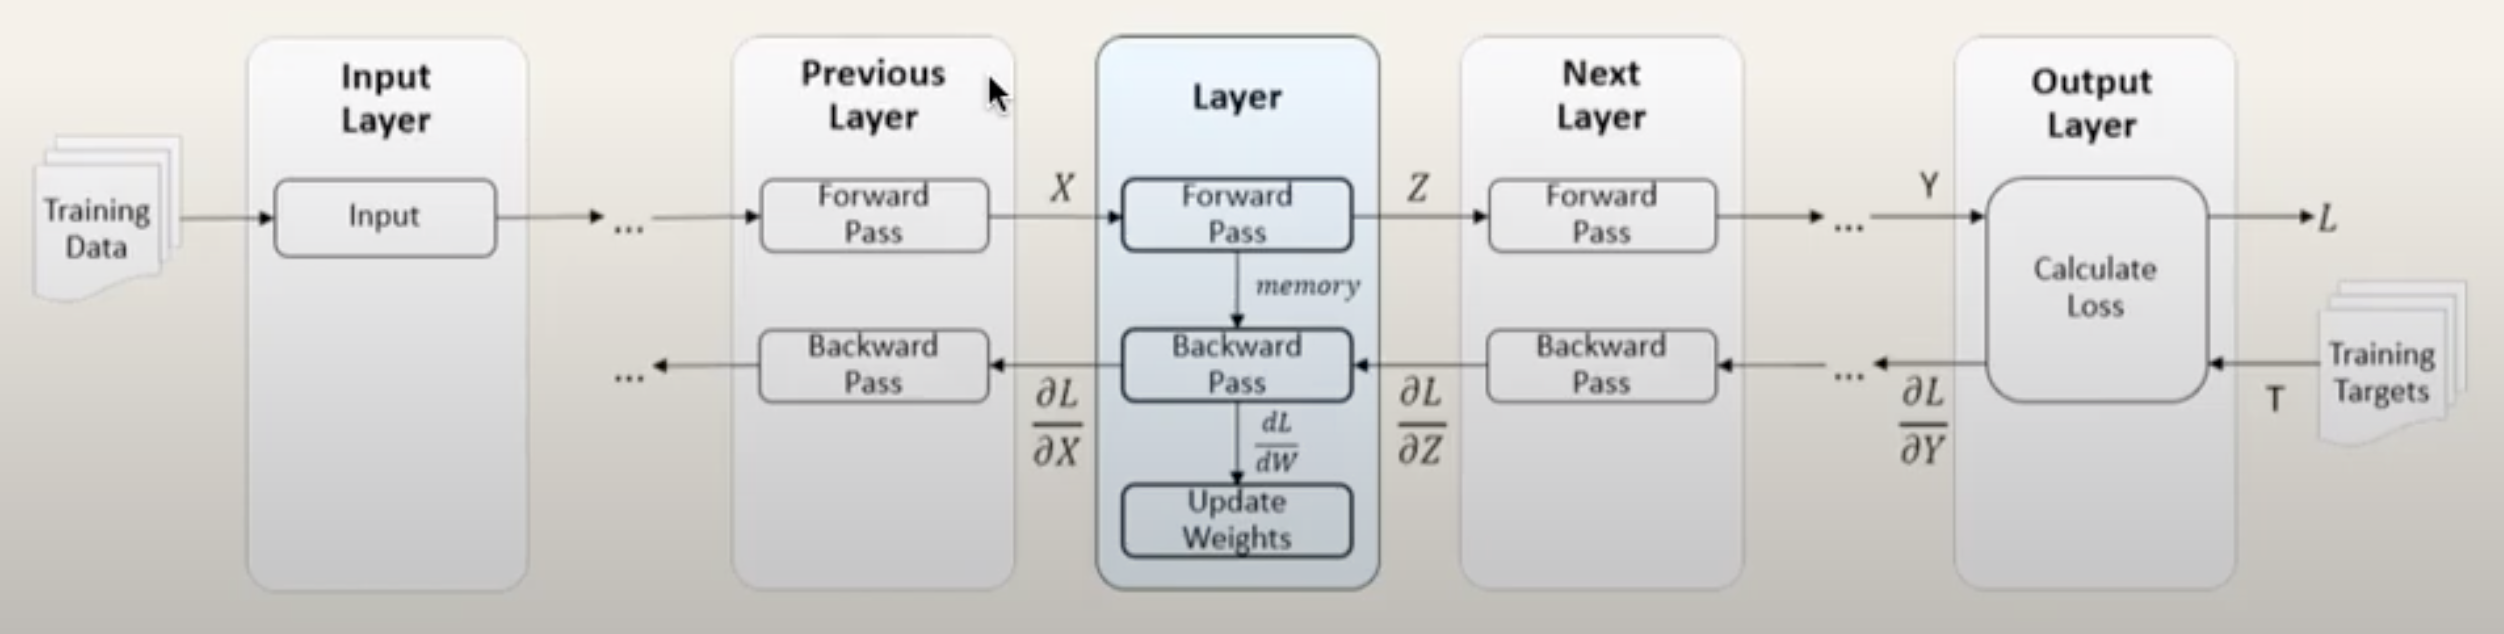
\includegraphics[scale = .35]{images/network_overview.png}}
\caption{Overview of BNN training, with an emphasis on forward and backward propagation.}
\label{fig:network_overview}
\end{figure}


Remember that weights are binarized in forward propagation. Below is a graph of the Sign(x) function used for deterministic binarization. Note that the derivative of the Sign function is zero almost everywhere, which makes it seem incompatible with the backward propagation method described above, where all gradients would equal zero. So how do BNNs get around this issue?


\begin{figure}
\centerline{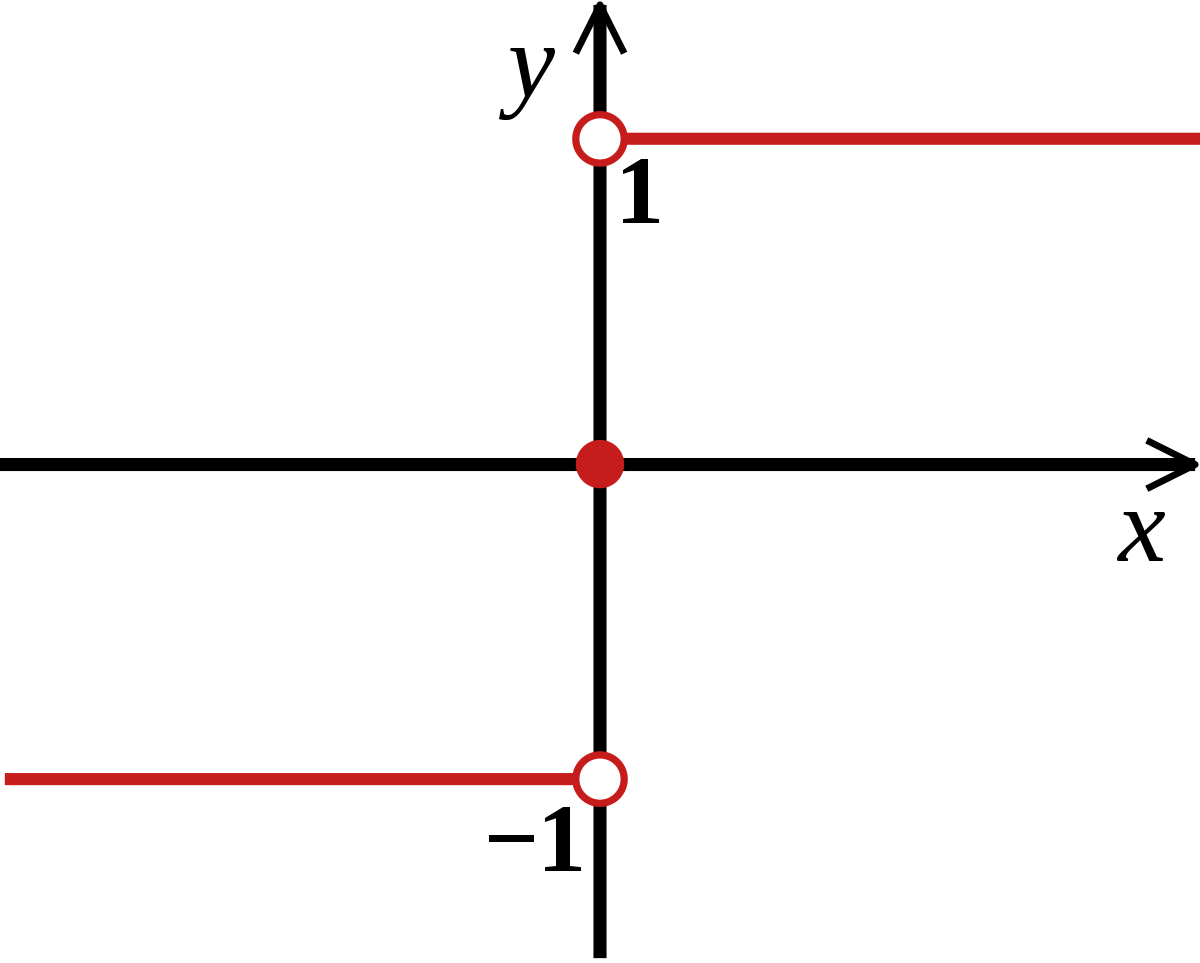
\includegraphics[scale = .15]{images/sign.png}}
\caption{Plot of Sign(x) for deterministic binarization. Note that the derivative of Sign(x) with respect to x is zero for nearly all x.}
\label{fig:sign}
\end{figure}


\subsection{Straight-Through Estimator}

Rather than use the analytical gradient of the loss with respect to the weights, we will calculate an estimate. In the context of backpropagation in BNNs, we will call this a straight through estimator (STE). In STEs, you set the incoming gradients to a threshold function equal to its outgoing gradients, disregarding the gradient of the threshold function itself. The figure below shows one layer of a BNN with Sign(x) as the activation function. Note that the top row is depicting a forward pass where Z are the incoming weights and Y are the outgoing weights (Y = Sign(Z)). The bottom row is depicting a backward pass on weights with respect to a loss function, L. On the backward pass, let \( g_Y = \frac{\partial L}{\partial Y} \) be the incoming derivative and let \( g_Z = \frac{\partial L}{\partial Z} \) be the analytical derivative (which would be 0 based on the analysis above). The STE computes \( g_Z \) to be \( g_Y \times \mathbb{1}_{\lvert Z \rvert \leq 1} \) where \( \times \) is element-wise multiplication with the indicator function. This is a difficult concept to grasp, but informally, this STE allows the binarization function to act as the identity function in the region around the current point (equivalent to using hard tanh function). %\\\\



\begin{figure}[h]
    \centering
    \begin{minipage}{0.45\textwidth}
        \centering
        \includegraphics[width=\textwidth]{images/STE.png}
        \caption{Zoomed-in look at one layer of BNN during training, showing use of STE during backpropagation.}
    \end{minipage}\hfill
    \begin{minipage}{0.37\textwidth}
        \centering
        \includegraphics[width=\textwidth]{images/hard_tanh.png}
        \caption{STE estimation of Sign function, as hard tanh function.}
    \end{minipage}
\end{figure}


% \begin{figure}[htbp]
% \centerline{\includegraphics[scale = .75]{STE.png}}
% \caption{Zoomed-in look at one layer of BNN during training, showing use of STE during backpropagation.}
% \label{fig2}
% \end{figure}

% \begin{figure}[htbp]
% \centerline{\includegraphics[scale = .55]{hard_tanh.png}}
% \caption{STE estimation of Sign function, as hard tanh function.}
% \label{fig2}
% \end{figure}

\newpage

\subsection{Backpropagation Pseudo Code}

The pseudo code for backward propagation of a BNN is shown below. We have also defined some important terms. In short, for each layer (except the last), we apply straight through estimation. We then perform a backwards pass for BatchNorm and calculate the estimated gradients of the weights with respect to the loss, and apply activation (the transpose step). In the second for loop, the weights are updated via gradient decent, and the gradients are passed left through the network.



\begin{itemize}
    \item C - loss function
    \item L - number of layers
    \item g - gradient (partial derivative)
    \item $s_k$ - activations before BatchNorm
    \item $a_k$ - activations after BatchNorm
    \item W - weight matrix
    \item superscript 'b' refers to a 'binarized' form of the variable
    \item $\theta$ - BatchNorm parameters
    \item $\eta$ - learning rate
\end{itemize}

\begin{figure}
\centerline{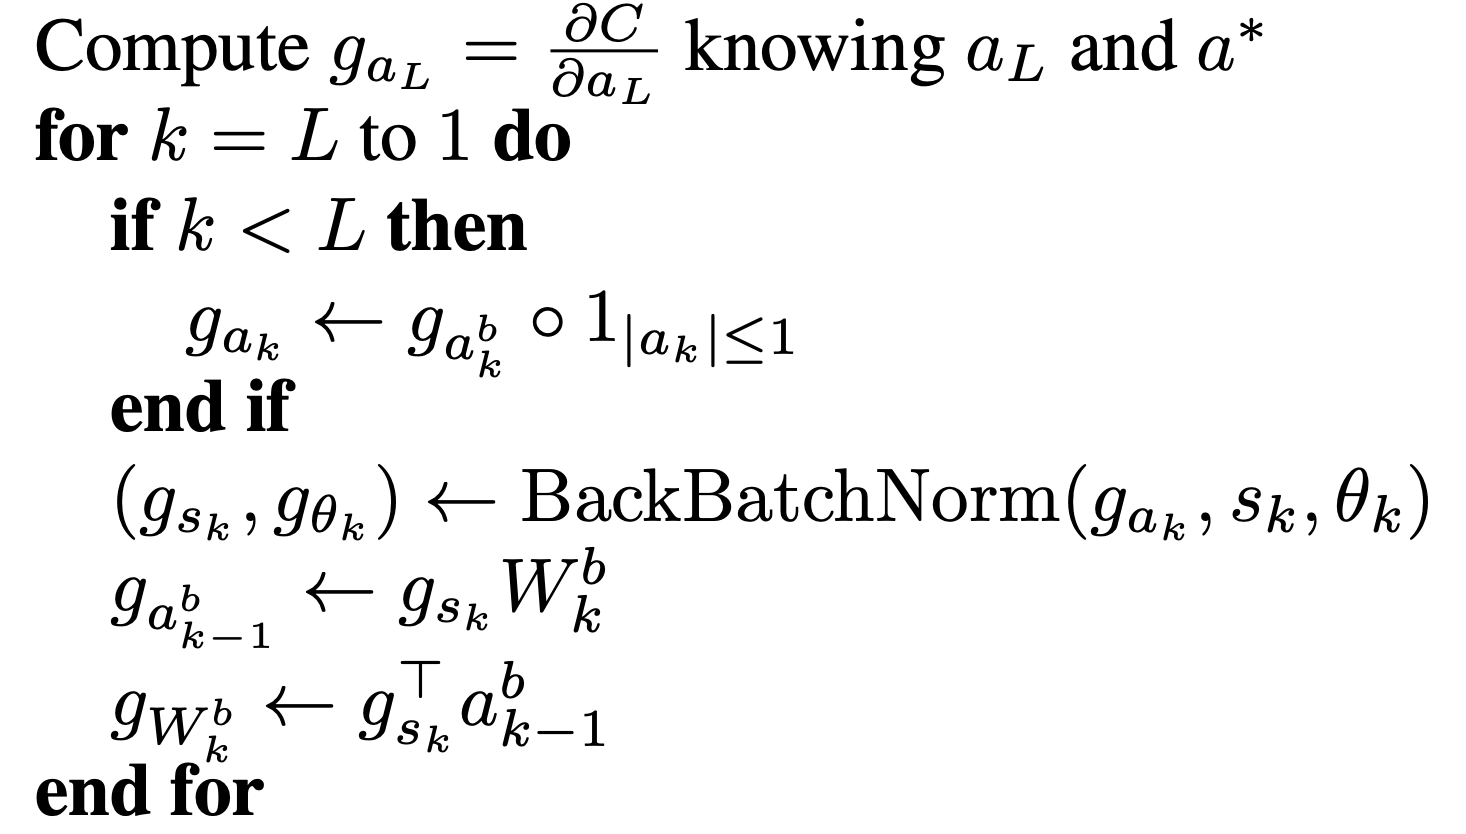
\includegraphics[scale = .35]{images/backprop_code.png}}
\centerline{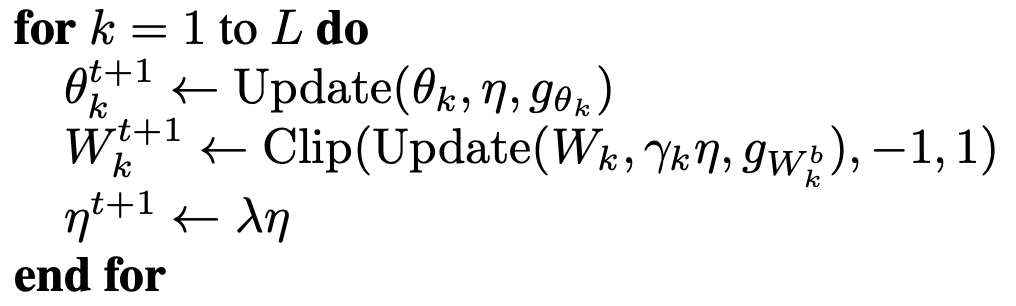
\includegraphics[scale = .50]{images/backprop_2.png}}
\caption{Pseudo code for BNN backward propagation}
\label{fig:backprop2}
\end{figure}

\section{Inference in BNNs}

This section serves as a review of how a BNN performs inference. At this stage, the BNN has been trained using multiple iterations of forward and backward propagation. Referencing (the first figure), an input to a BNN is a list (x vector). Let's say our goal is to predict the y. The network, having taken in a vector x, will perform the following operations to predict y (referred to as inference in neural networks). During the forward pass, the input data is processed through the network's layers, using the trained binary weights and activations. In BNNs, the standard dot product in the neurons is replaced by XNOR and popcount operations. These operations are much more efficient than floating-point multiplications and additions. At each layer, after the XNOR and bitcount operations, an activation function is applied (Sign). BNNs often use batch normalization to stabilize and speed up training. During inference, the learned parameters from batch normalization are used to normalize the activations. If the network includes pooling layers, convolutional layers, or other types of layers, these operate in a similar manner to their counterparts in traditional neural networks, but they are adapted to work with binary values. Finally, at the output layer, we receive our value for y (regression) or pass the final vector through typically a soft max (classification).

\subsection{Restatement of Advantage of BNNs, Limitations}
The key advantage of BNNs is that they require significantly less computational power and memory than traditional neural networks, making them well-suited for resource-constrained environments like mobile devices or embedded systems. However, the trade-off is that the binarization of weights and activations can lead to a loss in model accuracy, especially for complex tasks. In simple tasks such as number recognition, the BNN performs well, although requiring more layers than a full-precision NN. For complex tasks such as high-resolution image classificaiton and natural language processing, the lower expressiveness of the BNN may struggle to recognize complex patterns.
\nocite{bnn1, vid1, vid2, vid3, vid4, vid5, vid6}
% \nocite{stanford} \nocite{paper_explained} \nocite{review}

% \begin{thebibliography} {00}
% \bibitem{slides1} “Binary Neural Networks.” Lecture, n.d. https://docs.google.com/presentation/d/10lVe51Nh7w\_
% qmhlYheaYP1b8q6iOsutZ/edit#slide=id.p1. 
% \bibitem{bnn1}Courbariaux, Matthieu, Itay Hubara, Daniel Soudry, Ran El-Yaniv, and Yoshua Bengio. "Binarized neural networks: Training deep neural networks with weights and activations constrained to+ 1 or-1." arXiv preprint arXiv:1602.02830 (2016).
% \bibitem{vid1} EE545 (Week 10) “Binary Neural Networks” (Part I). YouTube. YouTube, 2020. https://www.youtube.com/watch?v=5K6ko3H\_ePg&amp;list=PLC89UNusI0eSBZhwHlGauwNq
% VQWTquWqp&amp;index=23&amp;t=338s. 
% \bibitem{vid2} EE545 (Week 10) “Binary Neural Networks” (Part II). YouTube. YouTube, 2020. https://www.youtube.com/watch?v=LcECmeFqbrI&amp;list=PLC89UNusI0eSBZhwHlGauwNq
% VQWTquWqp&amp;index=24. 
% \bibitem{vid3} EE545 (Week 10) “Binary Neural Networks” (Part III). YouTube. YouTube, 2020. https://www.youtube.com/watch?v=RC\_8bPv0uhM&amp;list=PLC89UNusI0eSBZhwHlGauwNq
% VQWTquWqp&amp;index=25. 
% \bibitem{vid4} EE545 (Week 10) “Binary Neural Networks” (Part IV). YouTube. YouTube, 2020. https://www.youtube.com/watch?v=P6sD8lI61Uk&amp;list=PLC89UNusI0eSBZhwHlGauwNq
% VQWTquWqp&amp;index=26. 
% \bibitem{vid5}EE545 (Week 10) “Binary Neural Networks” (Part V). YouTube. YouTube, 2020. https://www.youtube.com/watch?v=rHa0-mG5SuM&amp;list=PLC89UNusI0eSBZhwHlGauwNq
% VQWTquWqp&amp;index=27. 
% \bibitem{vid6} EE545 (Week 10) “Binary Neural Networks” (Part VI). YouTube. YouTube, 2020. https://www.youtube.com/watch?v=z8CclU5wKuY&amp;list=PLC89UNusI0eSBZhwHlGauwNq
% VQWTquWqp&amp;index=28. 
% \bibitem{stanford} Lin, Fang. Rep. XNOR Neural Networks on FPGA. CS231n: Deep Learning for Computer Vision, n.d. http://cs231n.stanford.edu/reports/2017/pdfs/118.pdf. 
% \bibitem{gpt} Ludvigsen, Kasper Groes Albin. “The Carbon Footprint of GPT-4.” Medium, July 18, 2023. https://towardsdatascience.com/the-carbon-footprint-of-gpt-4-d6c676eb21ae#:~:text=The\%20electricity\%20consumption\%20of\%20GPT\%2D4&amp;text=According\%20
% to\%20unverified\%20information\%20leaks,8\%20\%3D\%203\%2C125\%20servers\%20were\%20needed. 
% \bibitem{paper explained}Natsu. “Paper Explanation: Binarized Neural Networks: Training Neural Networks with Weights and Activations Constrained to +1 or −1.” Mohit Jain, August 16, 2018. https://mohitjain.me/2018/07/14/bnn/.
% \bibitem{slides2} "Neural Network.” Lecture, n.d. https://docs.google.com/presentation/d/1oC1Z\_LzzlGMdDCFpC
% 9rp6U2udwSpCaj-/edit#slide=id.p1. 
% \bibitem{medium} Ojha, Vikas Kuma. “Binary Neural Networks: A Game Changer in Machine Learning.” Web log. Geek Culture (blog). Medium, February 19, 2023. https://medium.com/geekculture/binary-neural-networks-a-game-changer-in-machine-learning-6ae0013d3dcb. 
% \bibitem{review}Yuan, Chunyu, and Sos S. Agaian. "A comprehensive review of binary neural network." Artificial Intelligence Review (2023): 1-65.

% \end{thebibliography}


% \nocite{*}
% \bibliographystyle{abbrv}
% \bibliography{ref}




% \end{document}


